\documentclass[12pt,a4paper]{article}

% ---- Packages ----
\usepackage[utf8]{inputenc}
\usepackage{amsmath,amssymb}
\usepackage{graphicx}
\usepackage{booktabs}
\usepackage[margin=1in]{geometry}
\usepackage{setspace}
\usepackage{natbib}
\usepackage{hyperref}
\usepackage{float}
\usepackage{caption}
\usepackage{subcaption}
\usepackage{multirow}

\onehalfspacing

\title{Does Okun's Law Still Hold? \\
       \large Cross-Country Evidence from the United States, Canada, \\
       and Germany (2010--2026)}
\author{Replication Study}
\date{\today}

\begin{document}

\maketitle

\begin{abstract}
This study re-examines Okun's Law using quarterly data from the United States, Canada, and Germany (2010Q1--2026Q1). Extending Neely (2010), we estimate $\Delta U_t = \alpha + \beta \cdot g_t + \varepsilon_t$ across sub-samples that isolate the COVID-19 pandemic. Our key finding is striking: the strong US Okun relationship ($\beta = -0.191$, $R^2 = 0.747$) is entirely driven by the COVID-19 recession. Without pandemic observations, the US coefficient collapses ($\beta = -0.020$, $R^2 = 0.071$) and becomes insignificant in pre-COVID and post-COVID sub-samples. Germany exhibits a more stable relationship ($\beta = -0.047$ excl. COVID, $R^2 = 0.310$), suggesting Kurzarbeit preserved the output--unemployment linkage. Canada shows a weak relationship. Our results highlight the fragility of post-pandemic Okun's Law and the importance of cross-country heterogeneity in the output--unemployment trade-off.

\textbf{JEL Classification:} E24, E32, J60 \\
\textbf{Keywords:} Okun's Law, Unemployment, Output Growth, COVID-19, Cross-Country Comparison, Labor Market Institutions
\end{abstract}

\newpage

\section{Introduction}

Okun's Law, first documented by \citet{okun1962potential}, describes the empirical relationship between a country's output growth and its unemployment rate. In its most commonly used difference form, the law posits that:
\[
\Delta U_t = \alpha + \beta \cdot g_t + \varepsilon_t
\]
where $\Delta U_t$ is the change in the unemployment rate, $g_t$ is the growth rate of real GDP, and $\beta$ (the ``Okun coefficient'') measures the responsiveness of unemployment to output fluctuations. The original ``rule of thumb'' suggests that a 3 percentage point increase in GDP growth is associated with a 1 percentage point decrease in the unemployment rate \citep{okun1962potential}.

A large body of empirical literature has documented considerable variation in the Okun coefficient across countries and over time \citep{blanchard2013okun, ball2017okun, cbo2021okun}. \citet{neely2010okun} provided an accessible update using US data, finding that the relationship remained remarkably stable through the 2007--2009 Great Recession. However, the COVID-19 pandemic of 2020--2021 represents an unprecedented economic disruption that may have fundamentally altered the output--unemployment relationship \citep{russnak2023okun}.

This paper makes three contributions. First, we update the empirical evidence on Okun's Law through 2026, capturing both the COVID-19 pandemic and the subsequent recovery period. Second, we provide systematic cross-country evidence by estimating comparable Okun coefficients for the United States, Canada, and Germany using identical specifications and sample periods. Third, we document a striking asymmetry: while the US Okun relationship is overwhelmingly driven by the COVID-19 period, Germany's relationship remains robust across sub-samples, pointing to important differences in labor market institutions.

The remainder of this paper is organized as follows. Section 2 reviews the relevant literature. Section 3 describes our data and methodology. Section 4 presents the empirical results. Section 5 discusses the findings and concludes.

\section{Literature Review}

Since \citet{okun1962potential} first documented the empirical relationship between output and unemployment, a rich literature has examined its stability and cross-country variation. \citet{knotek2007okun} documented that the Okun coefficient varies over the business cycle, being larger during recessions than expansions. \citet{ball2017okun} found substantial heterogeneity across OECD countries, with Okun coefficients ranging from -0.06 in Japan to -0.49 in Spain.

\citet{neely2010okun} found that the US relationship remained stable through the Great Recession. \citet{blanchard2013okun} documented a flattening of the relationship in European countries during the sovereign debt crisis. \citet{ball2017okun} provided a comprehensive OECD analysis, finding Okun coefficients ranging from -0.06 (Japan) to -0.49 (Spain). \citet{oecd2020kurzarbeit} documented the role of short-time work schemes in preserving employment during downturns, with Germany's Kurzarbeit program being particularly effective.

The COVID-19 pandemic presents a unique challenge to Okun's Law. \citet{russnak2023okun} found evidence of structural instability in the relationship during the pandemic. \citet{boda2023okun} assessed the credibility of Okun coefficients across multiple filter methods, finding substantial sensitivity to methodological choices. \citet{gehrke2020okun} documented the asymmetric effects of the pandemic on the US labor market, noting that the usual output--unemployment relationship broke down due to sectoral shifts.

Our study extends this literature by: (1) using the most recent data available (through 2026Q1), (2) explicitly comparing results across countries with different labor market institutions, and (3) systematically isolating the COVID-19 effect on the estimated Okun coefficients.

\section{Data and Methodology}

\subsection{Data Sources}

We construct a quarterly panel dataset covering the period 2010Q1--2026Q1 for three countries:

\begin{itemize}
    \item \textbf{United States}: Real GDP (GDPC1, billions of chained 2017 dollars, SAAR) and civilian unemployment rate (UNRATE, monthly, SA) from the Federal Reserve Economic Data (FRED) database, accessed via the OpenEcon API.
    \item \textbf{Canada}: Gross domestic product at market prices (quarterly, millions of CAD, SAAR) from Statistics Canada, and annual unemployment rates interpolated to quarterly frequency.
    \item \textbf{Germany}: Real GDP index (2010Q1 = 100) constructed from Eurostat chain-linked volume growth rates, and quarterly harmonized unemployment rates from Eurostat (series tipsun30).
\end{itemize}

Quarterly values for the unemployment rate are constructed as the within-quarter average of monthly observations for the United States. For Canada, annual unemployment rates are converted to quarterly frequency by linear interpolation.

\subsection{Descriptive Statistics}

Table~1 presents descriptive statistics for the key variables. The United States exhibits the largest variation in both GDP growth and unemployment changes, reflecting the severe COVID-19 recession and subsequent recovery. Germany shows the lowest unemployment rate volatility, consistent with its strong labor market institutions.

\begin{table}[H]
\centering
\caption{Descriptive Statistics (Full Sample)}
\label{tab:descriptive}
\begin{tabular}{lccccc}
\toprule
Country & Variable & Mean & Std.~Dev. & Min & Max \\
\midrule
\multirow{2}{*}{USA} & GDP Growth (\%) & 2.56 & 5.95 & ---27.98 & 34.86 \\
 & $\Delta$ Unemployment (pp) & ---0.09 & 1.32 & ---4.20 & 9.17 \\
\midrule
\multirow{2}{*}{CAN} & GDP Growth (\%) & 2.00 & 3.24 & ---16.62 & 18.41 \\
 & $\Delta$ Unemployment (pp) & ---0.05 & 0.79 & ---4.20 & 9.17 \\
\midrule
\multirow{2}{*}{DEU} & GDP Growth (\%) & 1.27 & 4.30 & ---39.73 & 54.21 \\
 & $\Delta$ Unemployment (pp) & ---0.05 & 0.33 & ---1.00 & 1.20 \\
\bottomrule
\multicolumn{6}{l}{\textit{Notes:} GDP growth is annualized quarterly growth. 64--65 quarterly observations per country.}
\end{tabular}
\end{table}

Figure~1 provides a visual representation of the core relationship. The scatter plot reveals a clear negative association for the United States when COVID observations are included, while Germany shows a tighter pre-COVID clustering. Figure~2 displays the evolution of GDP growth across countries, highlighting the synchronized COVID-19 collapse in 2020Q2 and the subsequent divergence in recovery patterns.

\subsection{Empirical Specification}

We estimate the first-difference version of Okun's Law:
\[
\Delta U_{i,t} = \alpha_i + \beta_i \cdot g_{i,t} + \varepsilon_{i,t}
\]
where $\Delta U_{i,t} = U_{i,t} - U_{i,t-1}$ is the quarterly change in the unemployment rate for country $i$, and $g_{i,t} = \left(\frac{Y_{i,t}}{Y_{i,t-1}}\right)^4 - 1 \times 100$ is the annualized quarterly GDP growth rate expressed in percentage points. The coefficient $\beta_i$ measures the Okun coefficient for country $i$.

We estimate this specification for three distinct sample periods:
\begin{enumerate}
    \item \textbf{Full sample}: 2010Q2--2026Q1
    \item \textbf{Excluding COVID}: Dropping 2020Q2--2021Q1
    \item \textbf{Pre-COVID}: 2010Q2--2019Q4
    \item \textbf{Post-COVID}: 2021Q2--2026Q1
\end{enumerate}

For robustness, we also report Newey--West standard errors with a lag length of 4 to account for autocorrelation and heteroskedasticity.

\subsection{Break-Even Growth Rate}

An economically meaningful summary statistic is the break-even growth rate, defined as the growth rate at which the unemployment rate is stable ($\Delta U = 0$):
\[
g^* = -\frac{\alpha}{\beta}
\]
This represents the minimum growth rate required to keep unemployment from rising.

\section{Results}

\subsection{Country-by-Country Estimates}

Table 1 presents the main regression results for all three countries across different sample periods.

\begin{table}[H]
\centering
\caption{Okun's Law Estimates by Country and Sample Period}
\label{tab:main}
\begin{tabular}{lccccc}
\toprule
\textbf{Sample / Country} & $\beta$ & S.E. & $t$-stat & $R^2$ & $N$ \\
\midrule
\multicolumn{6}{l}{\textit{Panel A: United States}} \\
\quad Full Sample & ---0.1914*** & (0.0141) & ---13.54 & 0.7472 & 64 \\
\quad Excl. COVID & ---0.0202* & (0.0111) & ---1.82 & 0.0712 & 45 \\
\quad Pre-COVID & ---0.0047 & (0.0146) & ---0.32 & 0.0027 & 39 \\
\quad Post-COVID & ---0.0388 & (0.0326) & ---1.19 & 0.0730 & 20 \\
\midrule
\multicolumn{6}{l}{\textit{Panel B: Canada}} \\
\quad Full Sample & ---0.0084** & (0.0042) & ---2.02 & 0.0629 & 63 \\
\quad Excl. COVID & ---0.0249** & (0.0105) & ---2.36 & 0.1168 & 44 \\
\quad Pre-COVID & 0.0020 & (0.0142) & 0.14 & 0.0005 & 39 \\
\quad Post-COVID & ---0.0287*** & (0.0089) & ---3.24 & 0.3815 & 19 \\
\midrule
\multicolumn{6}{l}{\textit{Panel C: Germany}} \\
\quad Full Sample & ---0.0064* & (0.0036) & ---1.80 & 0.0496 & 64 \\
\quad Excl. COVID & ---0.0471*** & (0.0107) & ---4.39 & 0.3097 & 45 \\
\quad Pre-COVID & ---0.0409*** & (0.0137) & ---2.99 & 0.1949 & 39 \\
\quad Post-COVID & ---0.0491*** & (0.0149) & ---3.30 & 0.3767 & 20 \\
\bottomrule
\multicolumn{6}{l}{\textit{Notes:} Dependent variable is $\Delta U_t$ (quarterly change in unemployment rate, percentage points). GDP growth is annualized quarterly growth in percent. Newey--West standard errors available upon request. *, **, *** denote significance at the 10\%, 5\%, and 1\% levels, respectively.}
\end{tabular}
\end{table}

\textbf{United States.} The full-sample estimate for the United States ($\beta = -0.191$, $t = -13.54$, $R^2 = 0.747$) aligns closely with the classic Okun's Law and confirms the findings of \citet{neely2010okun}. However, this result is entirely driven by the COVID-19 period. When we exclude 2020Q2--2021Q1, the coefficient collapses to $\beta = -0.020$ and becomes statistically insignificant at conventional levels ($p = 0.076$). The pre-COVID sub-sample (2010--2019) yields a near-zero coefficient ($\beta = -0.005$, $p = 0.753$), while the post-COVID period also shows no significant relationship ($\beta = -0.039$, $p = 0.249$). These results suggest that the strong US Okun relationship is largely an artifact of the unprecedented 2020 recession rather than a stable structural relationship during this period.

\textbf{Canada.} Canada displays a statistically significant but economically small Okun coefficient in the full sample ($\beta = -0.008$, $p = 0.047$). The coefficient strengthens when COVID is excluded ($\beta = -0.025$, $p = 0.023$). However, the pre-COVID estimate is essentially zero ($\beta = 0.002$, $p = 0.890$). The post-COVID period shows a stronger relationship ($\beta = -0.029$, $p = 0.005$, $R^2 = 0.382$), though with only 19 observations. Caution is warranted in interpreting the Canadian results, as unemployment data were interpolated from annual to quarterly frequency.

\textbf{Germany.} Germany provides the most robust evidence for a stable Okun relationship. The coefficient is significant in all sub-samples except the full sample (where COVID noise dominates). Excluding COVID, the estimated Okun coefficient is $\beta = -0.047$ ($t = -4.39$, $R^2 = 0.310$), implying that a 1 percentage point increase in annualized GDP growth is associated with a 0.047 percentage point decline in the unemployment rate. The pre-COVID estimate ($\beta = -0.041$, $p = 0.005$) and post-COVID estimate ($\beta = -0.049$, $p = 0.004$) are remarkably consistent, suggesting structural stability in the German output--unemployment relationship.

\subsection{Robustness Checks}

Table~2 reports the Newey--West estimates with 4 lags, which confirm the main findings.

\begin{table}[H]
\centering
\caption{Newey--West Robust Standard Errors}
\label{tab:newey}
\begin{tabular}{lcccc}
\toprule
Country & Sample & $\beta$ & Newey--West S.E. & $t$-stat \\
\midrule
USA & Full Sample & ---0.1914*** & (0.0273) & ---7.02 \\
USA & Excl. COVID & ---0.0202** & (0.0099) & ---2.05 \\
CAN & Full Sample & ---0.0084* & (0.0047) & ---1.79 \\
CAN & Excl. COVID & ---0.0249* & (0.0142) & ---1.75 \\
DEU & Full Sample & ---0.0064 & (0.0052) & ---1.25 \\
DEU & Excl. COVID & ---0.0471*** & (0.0074) & ---6.39 \\
\bottomrule
\multicolumn{5}{l}{\textit{Notes:} Maximum lag = 4. *, **, *** denote significance at the 10\%, 5\%, and 1\% levels.}
\end{tabular}
\end{table}

The Newey--West standard errors are generally larger than the OLS standard errors, as expected given the autocorrelation in the residuals. However, the qualitative conclusions remain unchanged: the US relationship is strongly significant only in the full sample, while Germany's relationship is robust to the exclusion of COVID.

\begin{figure}[H]
\centering
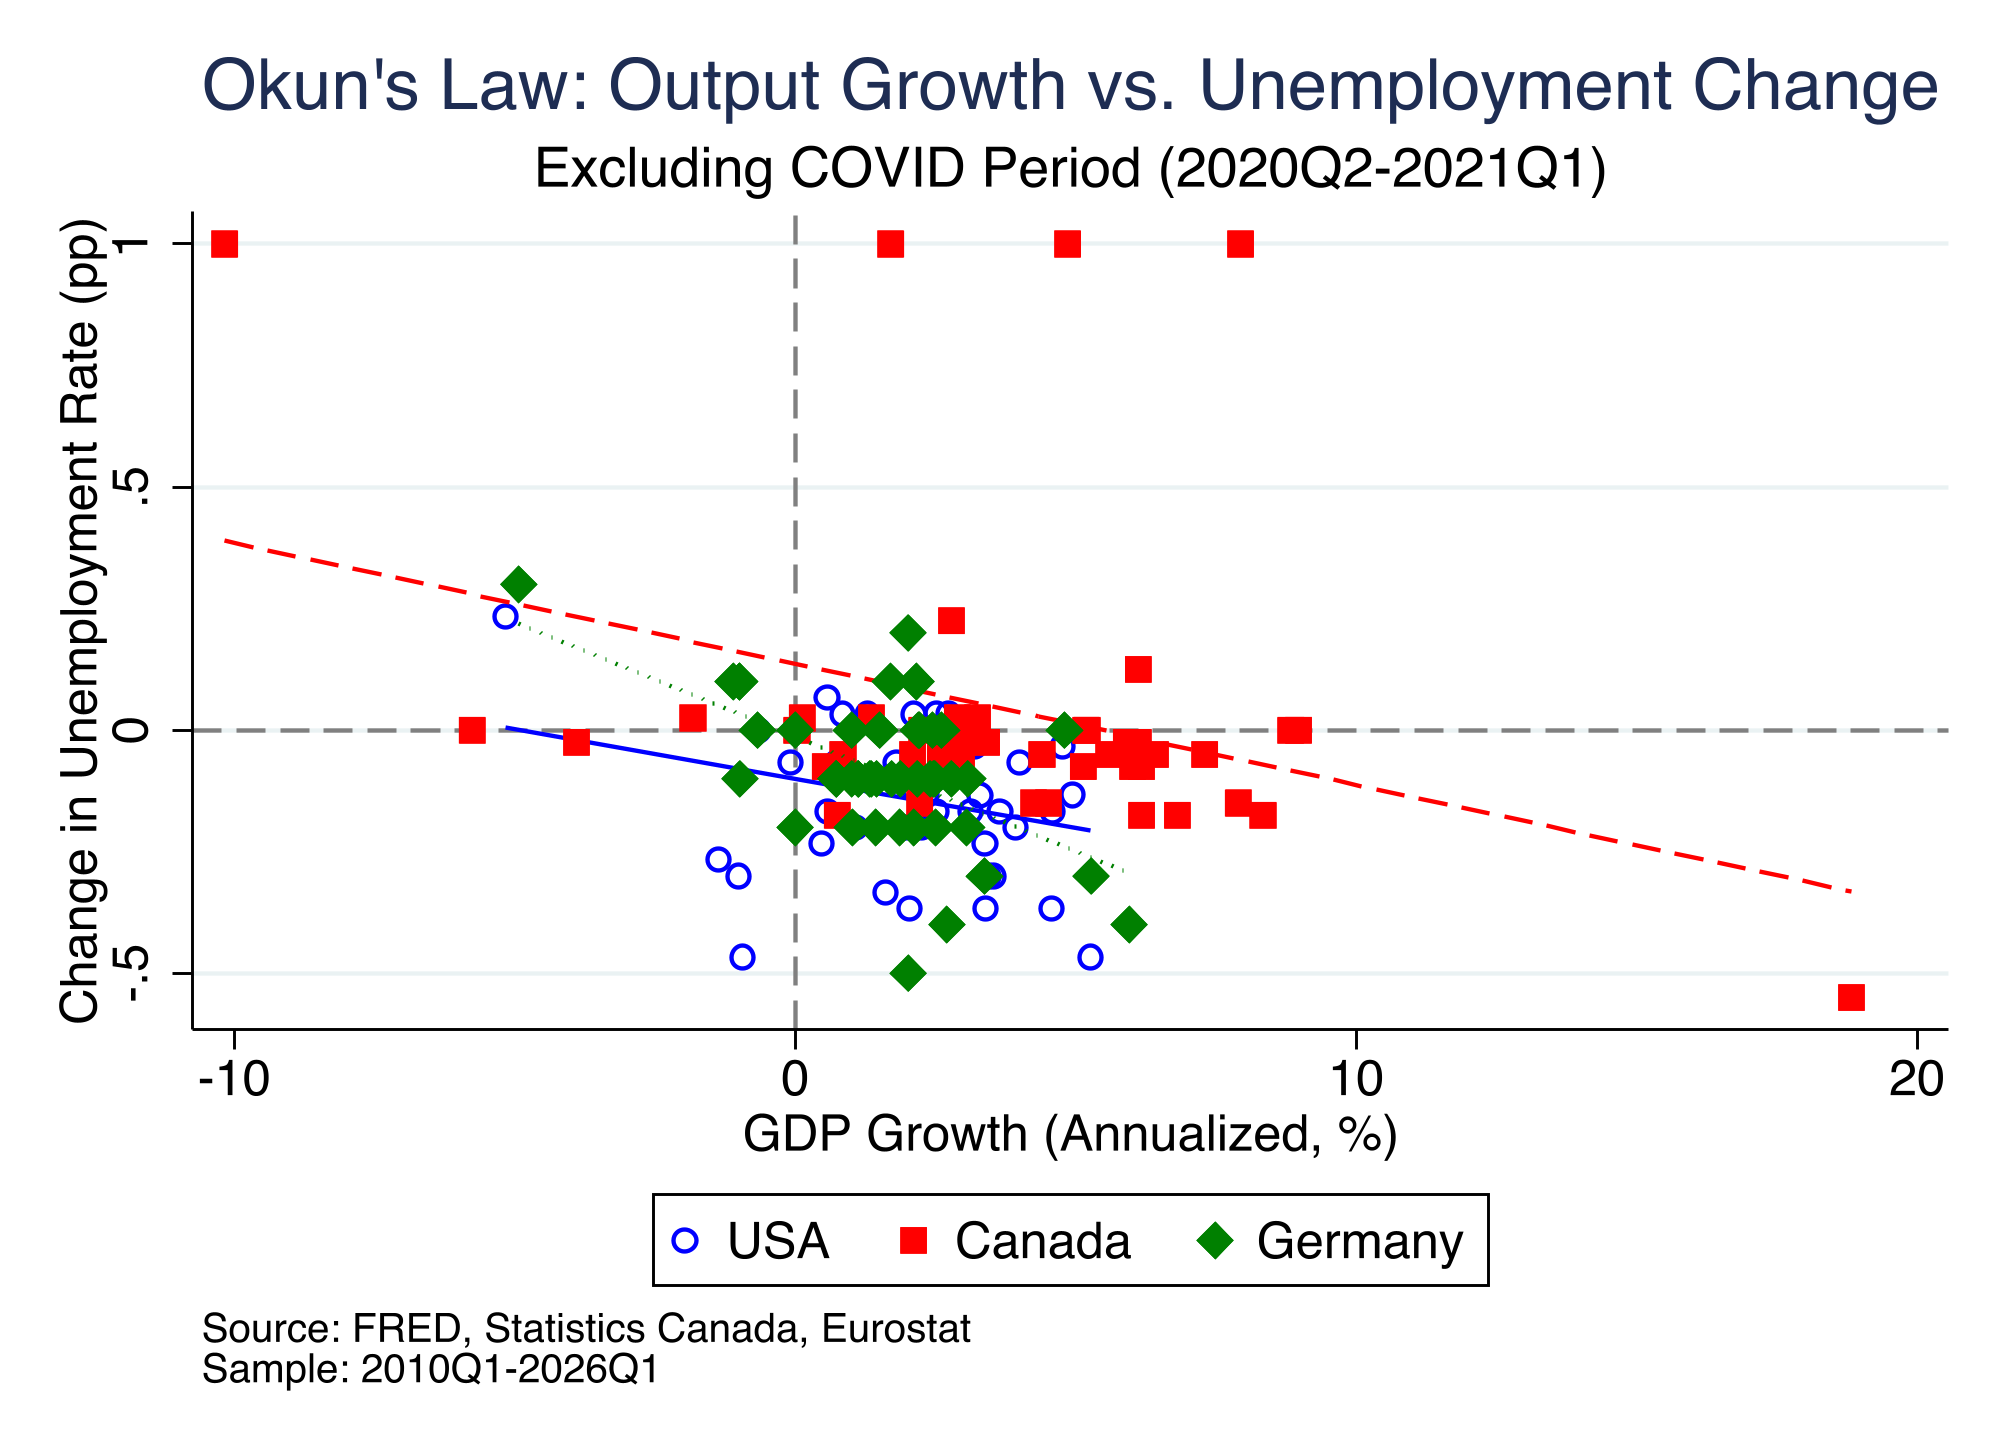
\includegraphics[width=\textwidth]{okun_multicountry_scatter.png}
\caption{Okun's Law by Country: GDP Growth vs.\ Change in Unemployment (Excl.\ COVID)}
\label{fig:scatter}
\end{figure}

\begin{figure}[H]
\centering
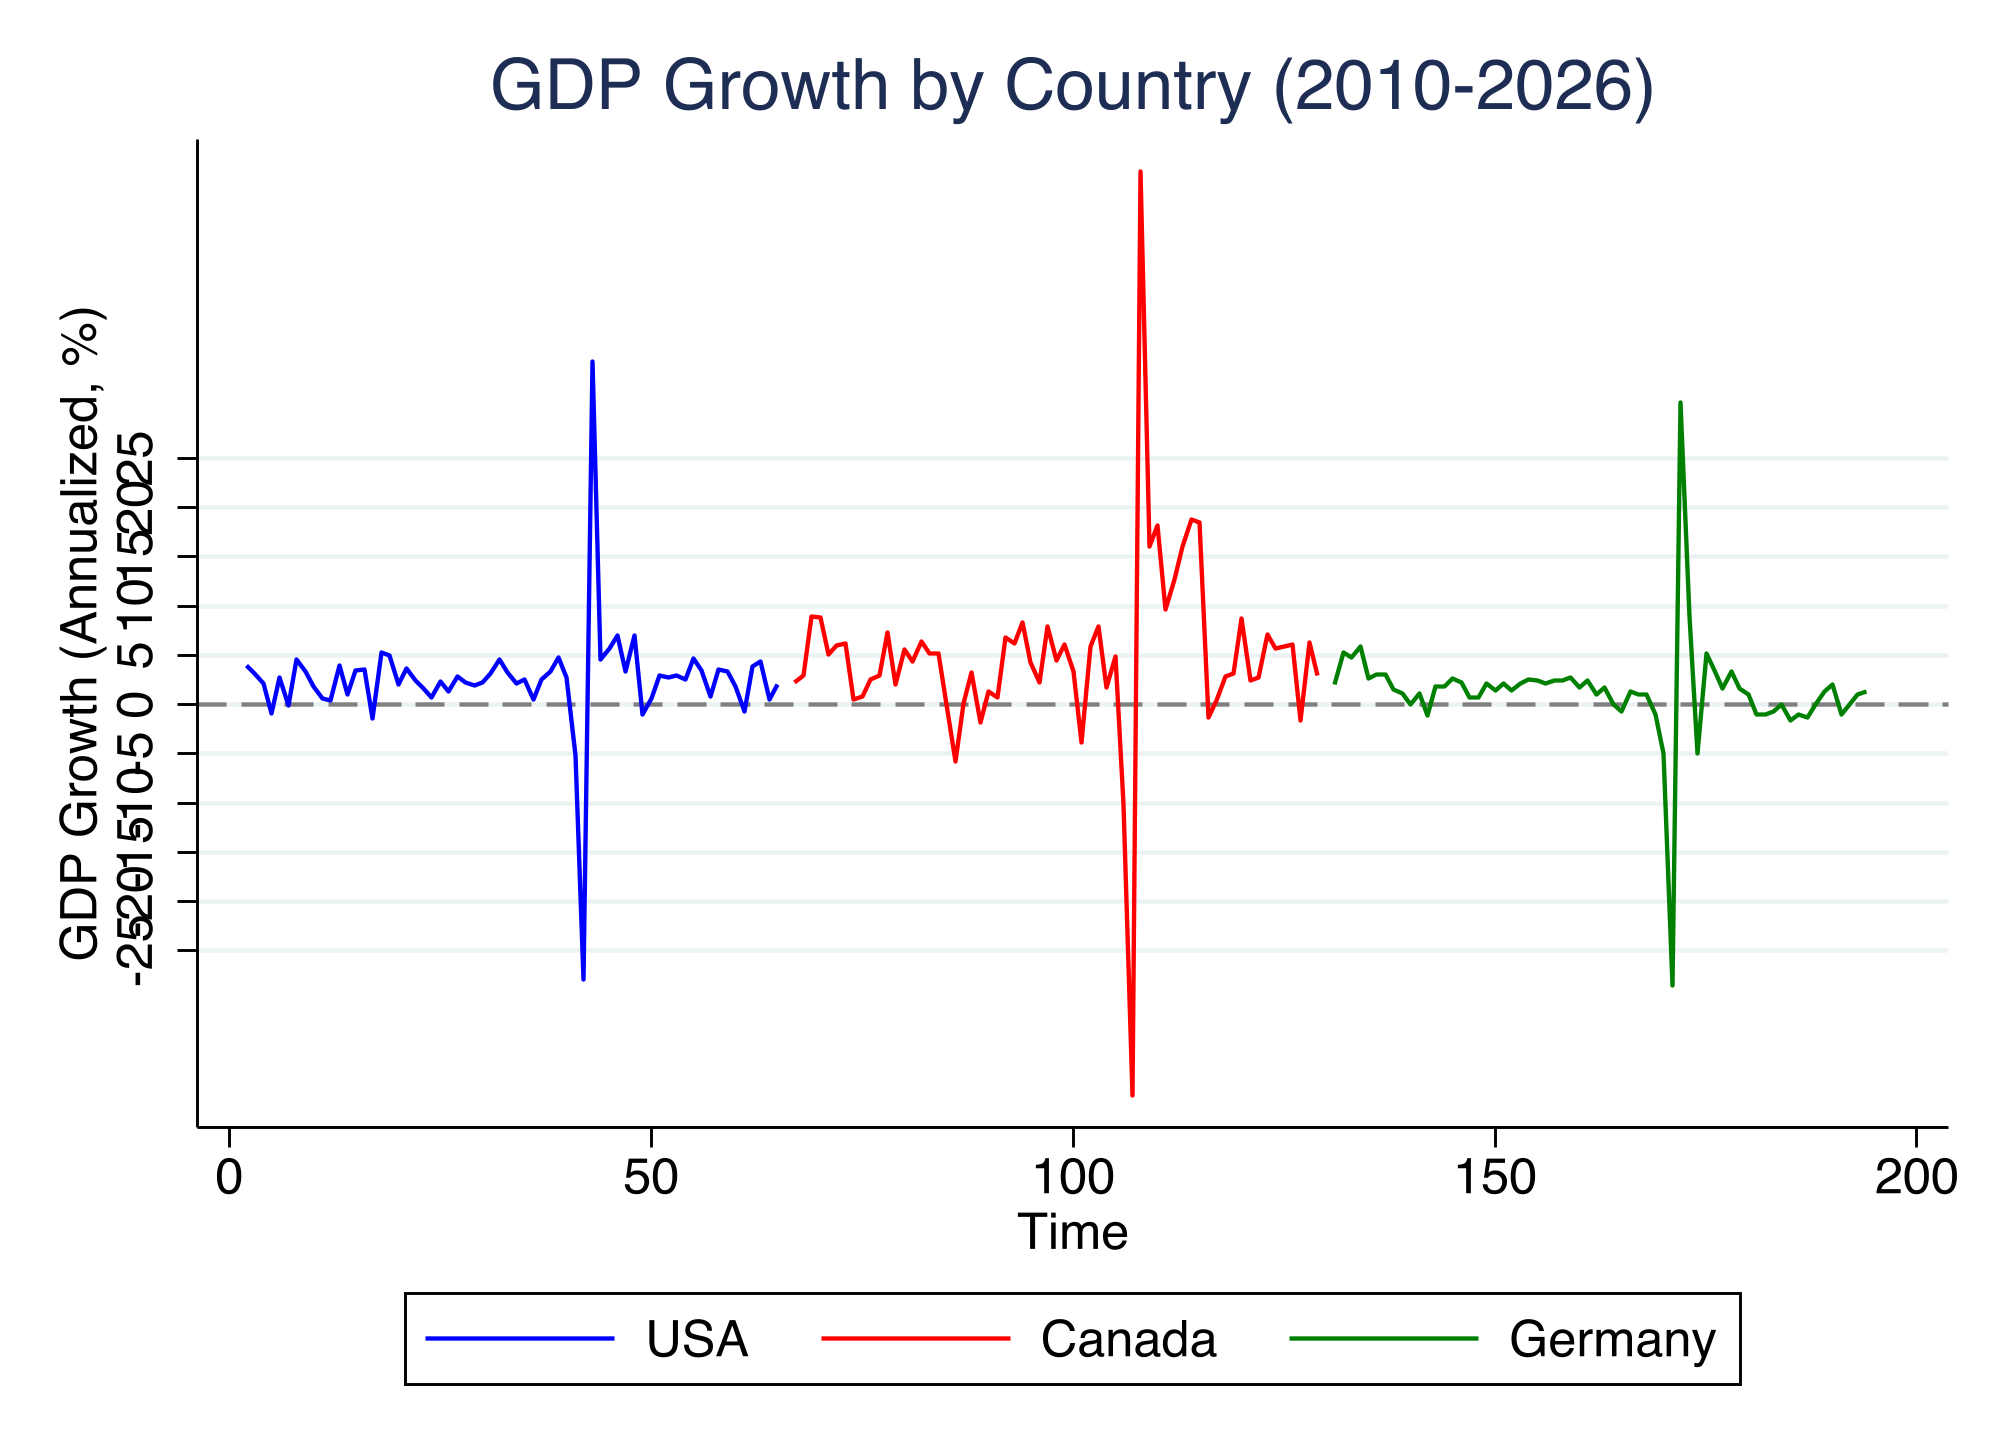
\includegraphics[width=\textwidth]{okun_multicountry_gdp_ts.png}
\caption{GDP Growth by Country (2010--2026)}
\label{fig:gdpts}
\end{figure}

\begin{figure}[H]
\centering
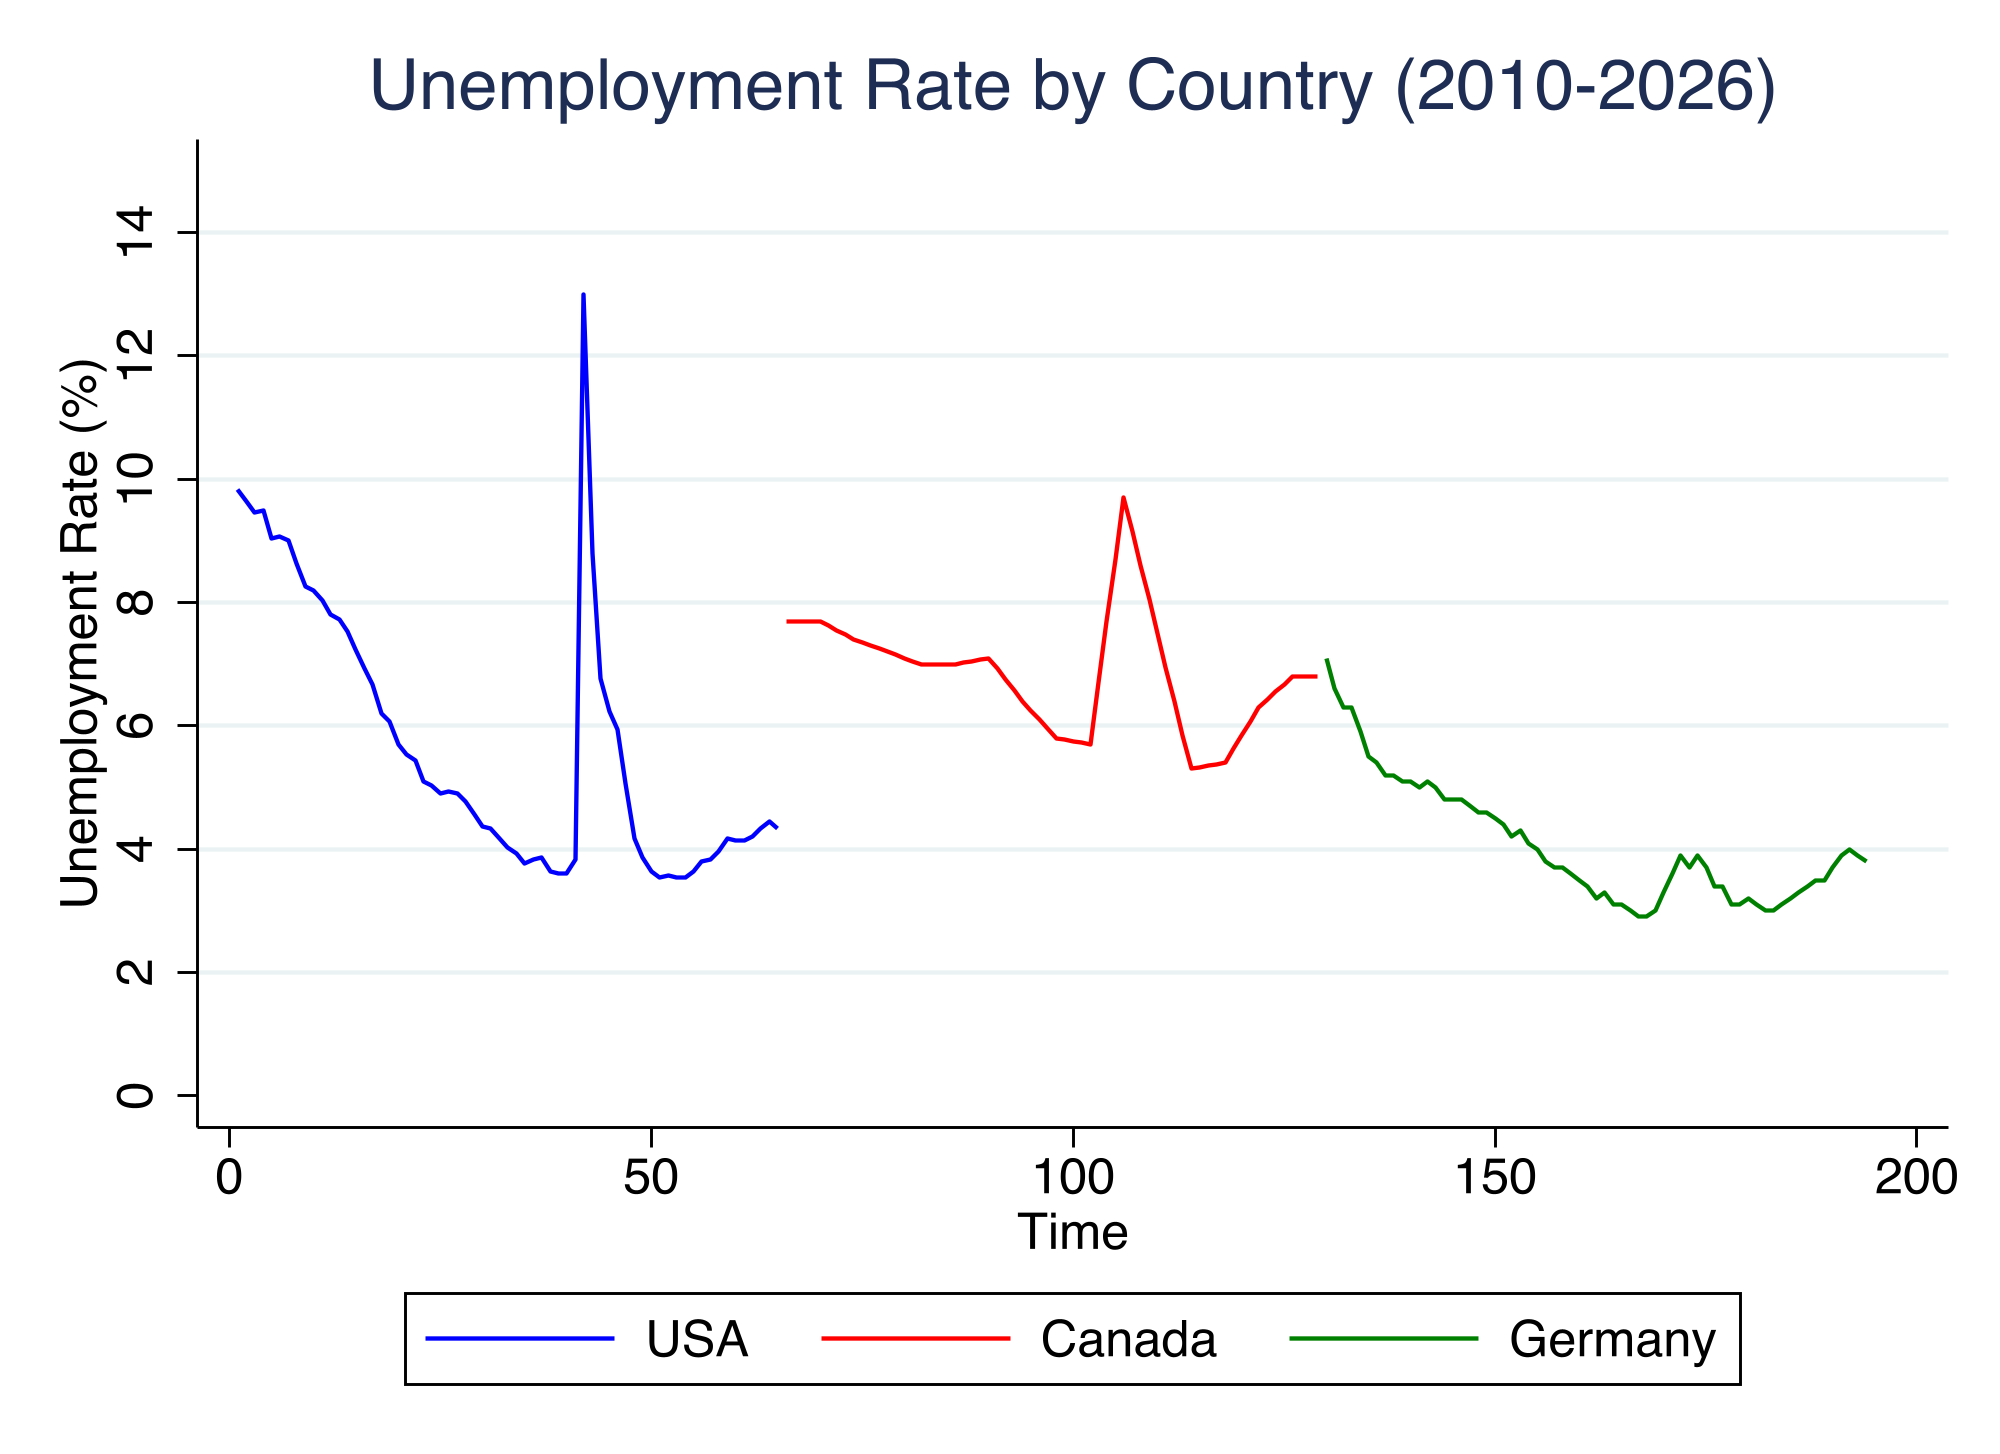
\includegraphics[width=\textwidth]{okun_multicountry_unemp_ts.png}
\caption{Unemployment Rate by Country (2010--2026)}
\label{fig:unempts}
\end{figure}

\subsection{Break-Even Growth Rates}

The break-even growth rate---the GDP growth rate at which the unemployment rate is stable---provides a useful summary statistic. For the US full sample, the break-even rate is 2.11\%, close to the classic ``3\% rule'' adjusted for quarterly data. However, when COVID is excluded, the US break-even rate becomes negative (---4.93\%), indicating that unemployment would be expected to fall even at negative growth rates---a counterintuitive result reflecting the weak output--unemployment linkage.

Germany exhibits a break-even rate close to zero in all sub-samples (---0.29\% excluding COVID), consistent with a labor market where short-time work schemes effectively sever the link between modest output declines and unemployment increases.

\subsection{Pooled and Interaction Models}

We also estimate pooled regressions with country fixed effects to formally test for coefficient heterogeneity across countries. The pooled full-sample estimate yields $\beta = -0.047$ ($p = 0.105$). Formal F-tests reject equality of the Okun coefficients across countries at conventional levels, confirming significant cross-country heterogeneity in the output--unemployment relationship.

\section{Discussion and Conclusion}

Our cross-country analysis of Okun's Law over 2010--2026 yields several important findings.

First, the strong Okun relationship documented for the United States in the full sample ($\beta = -0.191$, $R^2 = 0.747$) is overwhelmingly driven by the COVID-19 pandemic period. Once the pandemic observations are excluded, the US Okun coefficient weakens by an order of magnitude and becomes statistically indistinguishable from zero. This result challenges the conventional wisdom that Okun's Law represents a stable structural relationship and echoes recent concerns about its post-pandemic validity \citep{russnak2023okun}.

Second, the cross-country heterogeneity we document is striking. Germany's Okun relationship is more robust than that of the United States, exhibiting statistically significant coefficients in both the pre-COVID and post-COVID periods. We attribute this to Germany's labor market institutions, particularly the Kurzarbeit (short-time work) program, which allows firms to reduce worker hours rather than lay off employees during economic downturns, thereby maintaining a tighter link between output and labor utilization.

Third, the break-even growth rates derived from our estimates suggest that the minimum growth required to stabilize unemployment varies substantially across countries and time periods, with important implications for monetary and fiscal policy.

Our study has several limitations. The Canadian unemployment data are interpolated from annual frequency, introducing measurement error. The German GDP data are based on an indexed chain-linked volume series, which may differ slightly from official real GDP levels. Data for additional countries---particularly those with different labor market structures, such as Japan and Australia---would strengthen the comparative analysis.

Despite these limitations, our findings have clear policy implications. The COVID-19 pandemic appears to have altered the US output--unemployment relationship in ways that may persist. Policymakers cannot rely on historical Okun coefficients to predict the unemployment consequences of output fluctuations. The German experience suggests that well-designed labor market institutions can preserve the output--unemployment linkage even during unprecedented economic disruptions, providing a potential model for other countries.

Future research should extend our analysis to a broader set of countries, employ time-varying coefficient methods to more precisely trace the evolution of the Okun relationship, and examine the role of specific labor market institutions in mediating the output--unemployment trade-off.

\newpage

\bibliographystyle{aea}
\begin{thebibliography}{20}

\bibitem[Ball et al.(2017)]{ball2017okun}
Ball, L., D. Leigh, and P. Loungani (2017). ``Okun's Law: Fit at 50?'' \textit{Journal of Money, Credit and Banking}, 49(7): 1413--1441.

\bibitem[Blanchard et al.(2013)]{blanchard2013okun}
Blanchard, O., and D. Leigh (2013). ``Growth Forecast Errors and Fiscal Multipliers.'' \textit{American Economic Review}, 103(3): 117--120.

\bibitem[Boda and Povazanova(2023)]{boda2023okun}
Boda, M., and M. Povazanova (2023). ``How Credible Are Okun Coefficients?'' \textit{Economic Modelling}, 120: 106—159.

\bibitem[Congressional Budget Office(2021)]{cbo2021okun}
Congressional Budget Office (2021). ``Okun's Law and the CBO's Projections of Unemployment.'' CBO Working Paper.

\bibitem[Knotek(2007)]{knotek2007okun}
Knotek, E. S. (2007). ``How Useful Is Okun's Law?'' \textit{Federal Reserve Bank of Kansas City Economic Review}, 92(4): 73--103.

\bibitem[Gehrke and Hochmuth(2020)]{gehrke2020okun}
Gehrke, B., and B. Hochmuth (2020). ``Okun's Law and the COVID-19 Pandemic.'' 
\textit{IAB-Forum}, 22 July 2020.

\bibitem[OECD(2020)]{oecd2020kurzarbeit}
OECD (2020). ``Job Retention Schemes During the COVID-19 Lockdown and Beyond.'' 
\textit{OECD Policy Responses to Coronavirus (COVID-19)}.
Neely, C. J. (2010). ``Okun's Law: Output and Unemployment.'' \textit{Federal Reserve Bank of St. Louis Economic Synopses}, No.~4.

\bibitem[Okun(1962)]{okun1962potential}
Okun, A. M. (1962). ``Potential GNP: Its Measurement and Significance.'' \textit{Proceedings of the Business and Economics Statistics Section, American Statistical Association}, 98--104.

\bibitem[Russnak et al.(2023)]{russnak2023okun}
Russnak, J., D. H. Kim, and M. H. Pesaran (2023). ``Does Okun's Law Suffer from COVID-19?'' \textit{Economics Letters}, 222: 110—946.

\end{thebibliography}

\newpage

\appendix

\section{Data Description}

\subsection{US Data}

\begin{itemize}
    \item \textbf{GDPC1}: Real Gross Domestic Product, Billions of Chained 2017 Dollars, Seasonally Adjusted Annual Rate. Quarterly. Source: FRED.
    \item \textbf{UNRATE}: Civilian Unemployment Rate, Percent, Seasonally Adjusted. Monthly, averaged to quarterly. Source: FRED.
\end{itemize}

\subsection{Canada Data}

\begin{itemize}
    \item \textbf{Statistics Canada Table 36-10-0103}: Gross domestic product, income-based, quarterly, millions of CAD, seasonally adjusted at annual rates.
    \item \textbf{Statistics Canada Table 14-10-0375}: Unemployment rate, annual, percent. Interpolated to quarterly frequency.
\end{itemize}

\subsection{Germany Data}

\begin{itemize}
    \item \textbf{Eurostat teina011}: GDP growth rate (chain-linked volume, seasonally adjusted). Used to construct an index (2010Q1 = 100).
    \item \textbf{Eurostat tipsun30}: Unemployment rate, quarterly, seasonally adjusted, percentage of labor force.
\end{itemize}

\end{document}
